\documentclass[10pt]{article}
\usepackage[margin=16mm]{geometry}
\usepackage{graphicx,listings}
\lstset{basicstyle=\ttfamily\scriptsize,breaklines=true,columns=fullflexible}
\begin{document}
\section*{Native execution report: EXP-ECDLP-11c54d}
\noindent Observations only. Deterministic original worksheet reproduction/calibration; no scientific verdict, independent scientific review, attack claim or execution proof.\par\medskip
\noindent Run RUN-ECDLP-d9188a; hypothesis H-ECDLP-85fe43; goal GOAL-ECDLP-001.\par
\noindent Raw publication commit 1c9edbb900979bbff1d944f23bb24beae9325587.\par\medskip
Native status: output\_validated. Requested 1, output\_validated1, failed 0, timed out 0. Native elapsed 1.430079 seconds is derived as finished\_at minus started\_at. Measured manifest interval seconds=0.0980359609993684, child CPU seconds=0.067388, per-process RSS maximum bytes=15859712. Missing measurements are null, never zero. There is one deterministic worksheet, not a sampled inference; no uncertainty interval was recorded.\par\medskip
Execution commit 18098d6245946b3270908841f016ac9840825762; recorded dirty state True. Host/platform and Python are retained in report-data.json; detailed CPU model is missing.\par\medskip
Legacy identities EXP-ECDLP-3c166b / RUN-ECDLP-4a3ca0; raw bytes match original archive: True.
\subsection*{Recorded metrics}
\lstinputlisting{metrics.json}
\subsection*{Exact supervisor command and resource prefix}
\lstinputlisting{command.json}
\noindent Immutable record path: experiments/EXP-ECDLP-11c54d/runs/RUN-ECDLP-d9188a. Parameters, controls, null-seed semantics, full environment whitelist and source/input hashes are retained in report-data.json and the sealed run. Missing declared outputs: [].\par\medskip
Failure: None\par\medskip
This reports operational outputs only. Original predictions are historical calibration targets; repeated deterministic bytes are not fresh confirmatory data. Input seed remains null: no new random draw. Any original fixture/seed labels remain untouched. A null curve\_id does not certify an exact cross-repository subgroup identity. No discrete-log/decomposition certificate is claimed. The native checker is a source/control check, not independent scientific review. The first run's metadata Git utility failed to create threaded lstat under 256 MiB; its slot remains immutable. The subsequent three used the explicitly authorized process-local Git preload limit shown in command.json, with unchanged source/argv/scientific inputs and supervisor ceiling.\par\medskip
Canonical graph scope checked: knowledge/frontiers/ecdlp/ index and the batch's existing source/approval references. No scientific frontier, hypothesis status or isogeny graph was changed by these operational reproductions. A pipeline diagram is used because this experiment has one deterministic fixture, without two comparable experimental arms.\par
\begin{center}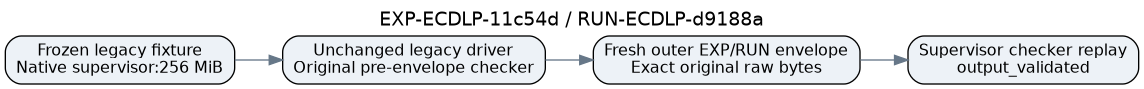
\includegraphics[width=\linewidth]{pipeline.png}\end{center}
\noindent Sources: ../../runs/RUN-ECDLP-d9188a/execution-receipt.json, manifest.yaml when present, raw-result.json when present, legacy-execution.json when present; report-data.json and runtime-diagnostic.json. All numbers are recorded measurements unless expressly labeled derived.
\end{document}
